% Snowflake Data Engineering — Chapter 7 | original manuscript draft
% Author: Arman Golbidi | Editorial snapshot: 22 October 2026
% Compile: xelatex -interaction=nonstopmode -halt-on-error Snowflake_Data_Engineering_Chapter_07.tex
% Trim: 178 x 254 mm; margins inside 23 mm / outside 17 mm / top-bottom 19 mm.
% Body: 10.75 pt / 13.65 pt leading = 1.27 line-height ratio; code: 8.75 pt.
\documentclass[11pt,twoside]{article}
\usepackage[paperwidth=178mm,paperheight=254mm,inner=23mm,outer=17mm,top=19mm,bottom=19mm,headheight=5mm,headsep=4mm,footskip=9mm]{geometry}
\usepackage{fontspec}
\setmainfont{LibertinusSerif-Regular.otf}[BoldFont=LibertinusSerif-Bold.otf,ItalicFont=LibertinusSerif-Italic.otf,BoldItalicFont=LibertinusSerif-BoldItalic.otf]
\setsansfont{LibertinusSans-Regular.otf}[BoldFont=LibertinusSans-Bold.otf,ItalicFont=LibertinusSans-Italic.otf]
\setmonofont{LibertinusMono-Regular.otf}[Scale=0.91]
\usepackage[english]{babel}
\usepackage{microtype}
\usepackage{setspace}
\setstretch{1.0}
\usepackage{titlesec,enumitem,tabularx,array,booktabs,needspace,fancyhdr,lastpage}
\usepackage[most]{tcolorbox}
\usepackage{tikz}
\usetikzlibrary{arrows.meta,positioning,fit,shapes.misc,calc}
\usepackage{listings}
\usepackage{xcolor}
\usepackage{hyperref}
\usepackage{amsmath}
\hypersetup{colorlinks=true,urlcolor=steelblue,linkcolor=steelblue,pdfauthor={Arman Golbidi},pdftitle={Snowflake Data Engineering - Chapter 7: Snowpipe, Streaming, and Real-Time Ingestion},pdfsubject={English technical book manuscript, sixth chapter, 178 x 254 mm}}
\definecolor{navy}{HTML}{15334A}
\definecolor{steelblue}{HTML}{17779B}
\definecolor{teal}{HTML}{12888A}
\definecolor{lightblue}{HTML}{ECF5F7}
\definecolor{papergray}{HTML}{F2F5F6}
\definecolor{inkgray}{HTML}{4A5862}
\definecolor{thinrule}{HTML}{CBD7DB}
\AtBeginDocument{\color{navy}\fontsize{10.75}{13.65}\selectfont}
\setlength{\parindent}{0pt}
\emergencystretch=2.5em
\setlength{\parskip}{3.3pt plus 0.7pt minus 0.6pt}
\setlist[itemize]{leftmargin=4mm,itemsep=1pt,topsep=2pt,parsep=0pt}
\setlist[enumerate]{leftmargin=5mm,itemsep=1pt,topsep=2pt}
\titleformat{\section}{\sffamily\bfseries\color{navy}\fontsize{14}{17}\selectfont}{}{0pt}{}
\titlespacing*{\section}{0pt}{8pt}{4pt}
\titleformat{\subsection}{\sffamily\bfseries\color{steelblue}\fontsize{10.8}{13}\selectfont}{}{0pt}{}
\titlespacing*{\subsection}{0pt}{5pt}{1pt}
\newcommand{\topic}[2]{\subsection*{#1\quad #2}}
\newcommand{\repo}[2]{\par\begingroup\fontsize{8.0}{9.6}\selectfont\sffamily\color{inkgray}\textbf{Project reference:} \href{#2}{#1}. \textit{Not independently executed; rights review pending.}\par\endgroup}
\newtcolorbox{insight}[1][]{enhanced,breakable,colback=lightblue,colframe=thinrule,boxrule=.45pt,arc=1.3mm,left=2.8mm,right=2.8mm,top=1.8mm,bottom=1.8mm,before skip=5pt,after skip=5pt,#1}
\newtcolorbox{whitebox}[1][]{enhanced,breakable,colback=papergray,colframe=thinrule,boxrule=.35pt,arc=1mm,left=2.6mm,right=2.6mm,top=1.5mm,bottom=1.5mm,before skip=4pt,after skip=5pt,#1}
\lstdefinestyle{chaptercode}{basicstyle=\ttfamily\fontsize{8.75}{10.7}\selectfont,backgroundcolor=\color{papergray},frame=single,framerule=.35pt,rulecolor=\color{thinrule},breaklines=true,columns=fullflexible,keepspaces=true,showstringspaces=false,aboveskip=5pt,belowskip=5pt,xleftmargin=2mm,xrightmargin=1mm,framexleftmargin=2mm,framexrightmargin=1mm}
\lstset{style=chaptercode}
\pagestyle{fancy}
\fancyhf{}
\fancyhead[LE]{\sffamily\fontsize{7.6}{9}\selectfont\color{inkgray}\textsc{Snowflake Data Engineering}}
\fancyhead[RO]{\sffamily\fontsize{7.6}{9}\selectfont\color{inkgray}\textsc{07 / Streaming Ingestion}}
\fancyfoot[LE,RO]{\sffamily\bfseries\fontsize{8.2}{9}\selectfont\color{steelblue}\thepage}
\fancyfoot[LO,RE]{\sffamily\fontsize{7.6}{9}\selectfont\color{inkgray}Arman Golbidi \quad | \quad Chapter 07}
\renewcommand{\headrulewidth}{0.35pt}
\renewcommand{\footrulewidth}{0pt}
\setcounter{page}{113}
\raggedbottom

% CHAPTER 07 ONLY, pages 113--132 in the planned book
\begin{document}
% PAGE 113 - INTRODUCTION
{\sffamily\bfseries\fontsize{9}{11}\selectfont\color{steelblue} CHAPTER 07 \hfill DATA ENGINEERING / CONTINUOUS INGESTION}\par\vspace{3mm}
{\sffamily\bfseries\fontsize{21.6}{25.5}\selectfont\color{navy} Snowpipe, Streaming, and\\Real-Time Ingestion}\par\vspace{2mm}
{\sffamily\fontsize{11.3}{14}\selectfont\color{steelblue} Build a pipeline whose freshness claims survive failures and replay}\par\vspace{4mm}
\begin{insight}\textbf{The alert was early. The evidence arrived late.}\par
At 10:05 an energy operator receives a grid-balancing alert. The dashboard still shows 09:45 generation figures, although sensors have transmitted readings every second. The team asks whether Snowflake is ``slow.'' But the missing time may be in a message broker, an object-storage batch, a cloud notification, a paused consumer, or the transformation after ingestion. The engineering question is not merely how rapidly bytes enter a table. It is \emph{how soon a trustworthy answer becomes visible to its intended reader}.\end{insight}
Chapter~5 designed reproducible file loading; Chapter~6 taught us to preserve, inspect and validate evolving event payloads. We now ask when files are enough and when continuously arriving rows justify a new ingestion contract. The Finland Energy Analytics Platform will retain its bronze--silver boundary, immutable event identity and UTC observation grain, but introduce event clocks, delivery offsets, operational visibility and recovery tests.
\begin{whitebox}\textbf{After this chapter you can:}
\begin{itemize}
\item choose scheduled \texttt{COPY INTO}, event-triggered Snowpipe or Snowpipe Streaming from measurable service needs;
\item explain cloud notifications, stages, pipes, streaming channels and checkpoint responsibilities;
\item separate source ordering, arrival ordering, revision precedence and query visibility;
\item exercise duplicate delivery, late observations, schema drift and transient failure safely;
\item present a defensible freshness and cost measurement plan without inventing cloud results.
\end{itemize}\end{whitebox}
\textbf{Prerequisites:} Chapters~3, 5 and 6; basic SQL and Python. The core lab is offline, with synthetic data. Live Snowflake examples are reviewed against vendor documentation but \emph{not executed in a customer account}. Region, edition, SDK version and consumption pricing must be rechecked before deployment.
\begin{center}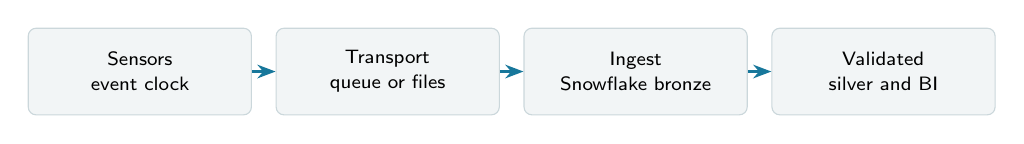
\begin{tikzpicture}[>=Stealth, every node/.style={font=\sffamily\fontsize{7.5}{9}\selectfont}, b/.style={draw=thinrule,rounded corners=1mm,fill=papergray,align=center,text width=26mm,minimum height=11mm}]
\node[b] (a) {Sensors\\event clock};\node[b,right=3mm of a] (b) {Transport\\queue or files};\node[b,right=3mm of b] (c) {Ingest\\Snowflake bronze};\node[b,right=3mm of c] (d) {Validated\\silver and BI};
\draw[-{Stealth},thick,steelblue](a)--(b);\draw[-{Stealth},thick,steelblue](b)--(c);\draw[-{Stealth},thick,steelblue](c)--(d);
\end{tikzpicture}\\{\fontsize{8}{9}\selectfont\color{inkgray}Figure 7.1. Freshness is an end-to-end property, not the ingestion API's name.}\end{center}
\newpage
% PAGE 114 - 7.1.1
\section*{7.1\quad Batch versus near-real-time versus streaming}
\topic{7.1.1}{Throughput and latency definitions}
A pipeline accepts units of work and exposes results. \textbf{Throughput} is the number of events, rows or bytes successfully processed per unit time; \textbf{latency} measures elapsed time for one particular work item. A system can exhibit excellent throughput while individual messages wait in a queue. Conversely, a tiny live demo can show low latency but collapse under an actual peak. Never infer one metric from the other.

Distinguish at least four clocks: \emph{event time}, when the device says the measurement applies; \emph{source publish time}, when the sender hands it to transport; \emph{ingest visibility time}, when the accepted bronze record can be queried; and \emph{business readiness time}, when validation and aggregation make it safe for the dashboard. A reliable SLA explicitly chooses the interval it measures, including its treatment of late source publication and failed arrivals.
\begin{whitebox}\textbf{Operational vocabulary}\par
\textbf{Event-to-visible age:} \(t_{\mathrm{visible}}-t_{\mathrm{event}}\). \textbf{Ingestion delay:} \(t_{\mathrm{visible}}-t_{\mathrm{publish}}\). \textbf{Business freshness:} how old the most recent \emph{accepted} observation is for a required key. \textbf{Backlog:} work accepted upstream but not yet committed and validated downstream.\end{whitebox}
\begin{lstlisting}[language=SQL,caption={Measure received-to-event age when both UTC timestamps are recorded.}]
SELECT technology,
  DATEDIFF('second', event_utc, received_utc)
    AS observed_source_age_seconds
FROM energy_telemetry_raw;
\end{lstlisting}
That query does \emph{not} measure actual Snowflake ingest service latency unless the receive timestamp was recorded at a reliably defined visibility boundary. The lab uses synthetic times precisely to exercise the formula; it makes no vendor speed claim. In production, collect enough rows for percentile statistics and stratify by provider, technology and hour: one median can hide an unacceptably slow tail.
\textbf{Decision check.} A stakeholder says ``we need real time.'' Ask: Freshness of which metric? Measured from which clock? What proportion must meet the target? How long may corrected values lag? These four answers determine architecture more usefully than the phrase itself.
\repo{P007: Snowflake time-series streaming guide}{https://github.com/Snowflake-Labs/sfguide-getting-started-with-time-series-using-snowflake-streaming-sis-ml-notebooks}
\newpage
% PAGE 115 - 7.1.2
\topic{7.1.2}{Batch, micro-batch, and continuous designs}
Scheduled batch loads move source snapshots or files at fixed intervals. They are easy to inspect, replay and reconcile; they add waiting time between arrivals. Micro-batching reduces that wait by processing frequent small groups, but every batch still needs discovery, serialization, commit and monitoring. Row-oriented streaming accepts new events without first requiring an object-storage file. None of these modes automatically produces a correct analytical table.

\begin{center}\small\renewcommand{\arraystretch}{1.15}\begin{tabularx}{\linewidth}{@{}p{25mm}X X@{}}\toprule
\textbf{Pattern}&\textbf{Strong fit}&\textbf{Primary burden}\\\midrule
Scheduled \texttt{COPY}&Hourly/daily immutable exports&Scheduler; batch boundaries\\
Snowpipe files&Frequent cloud-object arrivals&Notification plumbing; file lifecycle\\
Streaming API&Continuous event feeds&Checkpoints, retries, channel health\\\bottomrule
\end{tabularx}\\{\fontsize{8}{9.6}\selectfont\color{inkgray}Table 7.1. Select against workload requirements, not product branding.}\end{center}
Suppose a market report refreshes once an hour and source files arrive every fifteen minutes. Scheduled loading may be sufficient even if the source calls its service a ``stream.'' If operators need a sub-minute view of sensor fault indicators, waiting for objects to be created and discovered may be inappropriate. If the source only publishes once per hour, Snowpipe Streaming cannot invent more recent observations.

\textbf{A subtle architectural trap:} event frequency and decision frequency are different. Thousands of sensor events per second may be aggregated into five-minute operational windows, yet incident detection may depend on an instantaneous threshold. Split the design when workloads have distinct freshness and quality demands; do not send every raw event through the most expensive path merely because some consumers need fast alerts.
\begin{insight}\textbf{Design against two SLAs.}\par
The Finland energy example maintains \emph{bronze ingest visibility} and \emph{validated silver reporting readiness} as separate service objectives. Fast bronze ingestion with an hours-old silver watermark is still an operational failure for the analyst.\end{insight}
\textbf{Check.} Sketch two plans for a source producing one 2-MB object per minute: a scheduled load every fifteen minutes and event-triggered Snowpipe. Name every place a file can wait, and state which additional moving parts the second design introduces.
\newpage
% PAGE 116 - 7.1.3
\topic{7.1.3}{Costs, failure modes, and selection discipline}
Cost has both a metered and an engineering component. Batch loading typically consumes virtual-warehouse credits while the scheduled load runs. File-based Snowpipe uses Snowflake-managed ingestion services, with billing rules that are not identical to a user-managed warehouse. High-performance Snowpipe Streaming has a throughput-oriented ingestion billing model; actual charges depend on current account pricing and the volume measured by the service. Downstream SQL transformations, retained storage, notification infrastructure and monitoring may add costs in every option.

A useful comparison fixes the \emph{same accepted records} and the \emph{same business freshness objective}. Otherwise a cheap hourly batch and a continuously validated streaming system are solving different problems. Record: expected events/day; peak-to-mean ratio; average payload and file size; maximum acceptable loss and duplicate rate; replay horizon; human on-call time; retention; network egress; and idle-resource billing.
\begin{whitebox}\textbf{Why fast ingestion can be expensive operationally}\par
The fragile implementation fails when a client restarts, processes the same broker offset twice, mistakes ``sent'' for ``committed,'' loses its schema version, or publishes a late correction without adjusting the aggregate. Recovery and observation are part of streaming architecture, not optional polish.\end{whitebox}
\begin{lstlisting}[language=Python,caption={Design-time arithmetic; illustrative numbers, not vendor prices.}]
events_day = 86400 * 4          # four events per second
mean_bytes = 280                # application data estimate
estimated_GB_day = events_day * mean_bytes / 1e9
print(round(estimated_GB_day, 3))  # 0.097 GB/day
\end{lstlisting}
Even that number is not a bill: the accounting basis can exclude JSON structural bytes and include additional service classes. Avoid extrapolating a small simulator into a dollar forecast without the account's rate card.

\textbf{Decision procedure.} First confirm the source can deliver incremental data. Second define a p95/p99 freshness requirement and replay guarantee. Third run an identical input through two feasible patterns. Fourth measure downstream query visibility, data quality and metered usage. Finally document why the extra complexity is warranted. This chapter's controlled experiment provides the metrics framework; it does not claim to settle the choice for every team.
\newpage
% PAGE 117 - 7.2
\section*{7.2\quad Snowpipe architecture and auto-ingest concepts}
\topic{7.2.1}{Files, stages, and the PIPE object}
File-based Snowpipe is a managed service that uses a \texttt{PIPE} object to define a \texttt{COPY INTO} load from a stage. It loads new staged files without requiring you to schedule a virtual-warehouse \texttt{COPY} operation for each delivery. The pipe records loading instructions; storage integration and event publication are separate concerns. The pipeline still needs a stable file naming policy, predictable file formats and a contract for partial or rejected records.
\begin{lstlisting}[language=SQL,caption={File-based pipe definition; requires an approved external stage.}]
-- ENERGY_EVENTS_EXT and storage permissions are
-- provisioned separately. No cloud queue is created.
CREATE OR REPLACE PIPE ENERGY_FILE_PIPE
  AUTO_INGEST = FALSE AS
COPY INTO ENERGY_TELEMETRY_RAW
FROM @ENERGY_EVENTS_EXT
FILE_FORMAT = (TYPE = JSON);
\end{lstlisting}
\topic{7.2.2}{From cloud event to a visible row}
For auto-ingest, supported object-storage notifications announce new file objects; cloud-specific queue or subscription plumbing makes these announcements available to Snowflake. Snowpipe matches notifications to relevant staged paths and executes the pipe's load definition using managed compute. Visibility occurs later than a cloud's ``object created'' event; track both instants when diagnosing delay. An event is not the file itself, and a pipe declaration alone does not configure the notification service.
\begin{center}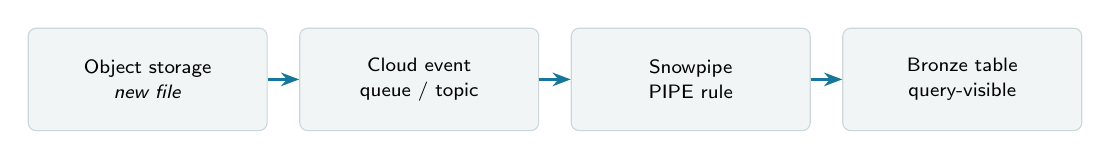
\begin{tikzpicture}[>=Stealth,every node/.style={font=\sffamily\fontsize{7.5}{9}\selectfont},b/.style={draw=thinrule,fill=papergray,rounded corners=1mm,align=center,text width=28mm,minimum height=13mm}]
\node[b](a){Object storage\\\emph{new file}};\node[b,right=4mm of a](b){Cloud event\\queue / topic};\node[b,right=4mm of b](c){Snowpipe\\PIPE rule};\node[b,right=4mm of c](d){Bronze table\\query-visible};
\draw[->,thick,steelblue](a)--(b);\draw[->,thick,steelblue](b)--(c);\draw[->,thick,steelblue](c)--(d);
\end{tikzpicture}\\{\fontsize{8}{9}\selectfont\color{inkgray}Figure 7.2. Events trigger file discovery; files hold the source records.}\end{center}
\topic{7.2.3}{Arrival and load observability}
\texttt{SYSTEM\$PIPE\_STATUS} exposes operational state for a pipe, including notification-related fields for auto-ingest where available. Load history and error notifications give different views: do not treat an empty error log as proof of complete source delivery. Reconcile file manifests against accepted rows and keep rejected-record provenance.
\repo{P048: Auto-ingest demonstration}{https://github.com/Snowflake-Labs/sfguide-twitter-auto-ingest}
\newpage
% PAGE 118 - 7.3
\section*{7.3\quad Cloud event notifications and staged files}
\topic{7.3.1}{Event topics, queues, and subscriptions}
An object-store notification announces that a file has appeared or changed. Depending on cloud provider, configuration can involve S3 events and queues, Azure event infrastructure or Google Cloud Pub/Sub; Snowflake's integration instructions are cloud-specific. Specify an event subscription restricted to the intended path and event type. Broad notifications can waste work, expose sensitive object names or route unrelated files to the same ingestion path.
\topic{7.3.2}{Storage integration as a trust boundary}
A stage tells Snowflake \emph{where} to look; storage integration determines which permitted identity may read it. Principle of least privilege applies to both the Snowflake role that creates or operates pipes and the cloud identity authorized to access objects. Prefer dedicated paths per environment, and avoid embedding cloud access keys in book code. Before deployment, check region constraints and organizational data-residency policy.
\begin{whitebox}\textbf{Common failure: notifications succeed, access fails.}\par
Cloud monitoring shows the object-created event was published, yet no data appear. The pipe may lack rights to read the object, the stage may target a different prefix, the file format may reject records, or a queue permission may block delivery. Diagnose \emph{object access}, \emph{notification receipt}, \emph{copy execution}, and \emph{silver validation} as separate gates.\end{whitebox}
\topic{7.3.3}{Duplicates, replays, and delivery assumptions}
Cloud notifications may be repeated or delayed; object keys may be reused; producers may overwrite existing keys. A safe publication policy uses immutable object names that encode source partition and batch identity. Do not claim that a repeated notification always adds duplicate table rows; Snowflake tracks file loading in supported workflows, but its load metadata retention and reloading behavior have limits. Your source-level deduplication and reconciliation policy remains necessary.
\begin{lstlisting}[language=SQL,caption={Inspect a configured pipe without changing data.}]
SELECT SYSTEM$PIPE_STATUS('ENERGY_FILE_PIPE');
-- Inspect notification queue state and error fields
-- in context of this account's cloud provider.
\end{lstlisting}
\textbf{Recovery drill.} A cloud notification is lost while the source file remains in object storage. Demonstrate a bounded, audited backfill procedure based on a manifest and ingestion history, not a blind ``force reload every file'' script. Document who may approve a replay and which analytical keys are protected from double-counting.
\repo{P056: Terraform Snowpipe cloud plumbing}{https://github.com/Snowflake-Labs/terraform-snowflake-snowpipe-aws}
\newpage
% PAGE 119 - 7.4.1
\section*{7.4\quad Snowpipe Streaming fundamentals}
\topic{7.4.1}{Architecture: classic and high-performance paths}
\textbf{Snowpipe Streaming} accepts event records directly through a supported ingest client rather than first discovering a staged file. As of this manuscript's documentation checkpoint, two architectural families matter. The \emph{classic} approach uses its original SDK, channel conventions and operational limitations. The \emph{high-performance} approach uses newer SDK/REST interfaces and a server-side \texttt{PIPE} to accept and, where configured, transform streamed rows. They are not merely two names for identical code. Follow the documentation for the client and architecture actually selected.
\begin{center}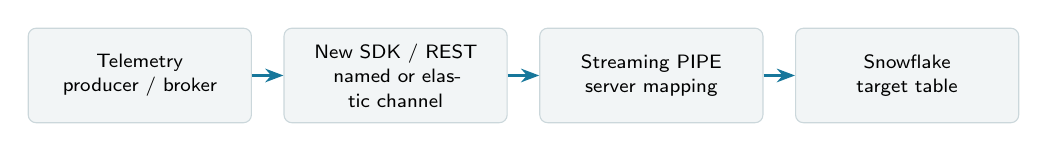
\begin{tikzpicture}[>=Stealth,every node/.style={font=\sffamily\fontsize{7.3}{8.8}\selectfont},b/.style={draw=thinrule,rounded corners=1mm,fill=papergray,align=center,text width=26mm,minimum height=12mm}]
\node[b] (a) {Telemetry\\producer / broker};\node[b,right=4mm of a](b){New SDK / REST\\named or elastic channel};\node[b,right=4mm of b](c){Streaming PIPE\\server mapping};\node[b,right=4mm of c](d){Snowflake\\target table};
\draw[->,thick,steelblue](a)--(b);\draw[->,thick,steelblue](b)--(c);\draw[->,thick,steelblue](c)--(d);
\end{tikzpicture}\\{\fontsize{8}{9.2}\selectfont\color{inkgray}Figure 7.3. High-performance streaming uses a server-side pipe entry point.}\end{center}
In the high-performance architecture, you can define a named pipe for custom mapping, or use a supported default-pipe workflow. Where the architecture and SDK support them, \emph{named channels} allow explicit offset tracking. Some interfaces also offer \emph{elastic channels} with a different delivery model. Do not transfer an exactly-once claim from one channel mode to another. Those terms have consequences for retries and deduplication.

\textbf{The database boundary matters.} A successful SDK submission, a committed channel offset and a business-valid silver row are three distinct states. For the energy platform, raw telemetry carries event identity, source partition/offset, original event time, producer schema version and processing status. Transformations that compute publication-ready MWh totals occur downstream, where duplicates and revisions can be resolved with domain rules.
\repo{P068: Snowpipe Streaming SDK examples}{https://github.com/snowflakedb/snowpipe-streaming-sdk-examples}
\newpage
% PAGE 120 - 7.4.2
\topic{7.4.2}{Rows versus files: the engineering boundary}
File-based Snowpipe and row-based Snowpipe Streaming can both produce bronze records, but the delivery units differ. A file pipeline needs object naming, object lifecycle, cloud notification integration and file-load auditing. A row pipeline needs channel identity, source offsets, client resilience, schema mapping and row-error behavior. Shared downstream obligations include time semantics, privacy, reconciliation, data quality and cost attribution.
\begin{center}\renewcommand{\arraystretch}{1.13}\begin{tabularx}{\linewidth}{@{}p{31mm}XX@{}}\toprule
\textbf{Dimension}&\textbf{Snowpipe files}&\textbf{Streaming API}\\\midrule
Transport unit&Cloud object&Row / client batch\\
Primary identity&File path + load state&Source event and channel offset\\
Discovery&Notification or refresh&Client submission\\
Recovery&Manifest, load history, backfill&Checkpoint, replay, row errors\\
Typical source&Periodic exports&Broker, IoT, CDC event stream\\\bottomrule\end{tabularx}\\{\fontsize{8}{9.5}\selectfont\color{inkgray}Table 7.2. Both options need explicit correctness contracts.}\end{center}
Do not confuse Snowpipe Streaming with the SQL \texttt{STREAM} object introduced later in Chapter~8. The former is an \emph{ingestion interface}; the latter tracks changes to a Snowflake table for downstream consumption. Likewise, receiving CDC messages from an upstream database is not the same as using a Snowflake change-tracking stream. Similar vocabulary hides different ownership and failure modes.

\begin{insight}\textbf{Why not stream everything?}\par
An hourly regulator report that must be signed off against immutable batches benefits from file manifests and bounded reconciliation. A high-frequency sensor feed requiring rapid anomaly identification may prefer a streaming client, but if the business reprocesses daily for reporting, it can still retain an immutable archive for audit. Mixed paths can coexist when their acceptance and reconciliation rules are clear.\end{insight}
\textbf{Check.} Compare a source sending 10,000 tiny files per hour with a source sending 10,000 events per hour over a broker. Which ingestion unit is natural in each case? What changes in operational burden when you force one source into the other's delivery unit?
\repo{P070: Official Snowflake Kafka connector}{https://github.com/snowflakedb/snowflake-kafka-connector}
\newpage
% PAGE 121 - 7.4.3
\topic{7.4.3}{Supported interfaces and deployment checks}
For the high-performance architecture, official Snowflake materials document a newer Java/Python SDK family and REST endpoints, with interface-specific behavior for channel operations. Availability, implementation limits, SDK APIs, region coverage and throughput ceilings are versioned product facts, not permanent design axioms. Freeze exact library versions and check the current documentation immediately before execution or publishing.
\begin{lstlisting}[language=SQL,caption={Illustrative high-performance streaming pipe syntax.}]
CREATE OR REPLACE PIPE ENERGY_EVENTS_STREAM_PIPE AS
COPY INTO ENERGY_TELEMETRY_RAW
  (EVENT_ID, TECHNOLOGY, EVENT_UTC,
   ENERGY_MWH, REVISION)
FROM (SELECT
  $1:event_id::VARCHAR,
  $1:technology::VARCHAR,
  TRY_TO_TIMESTAMP_NTZ($1:event_utc::VARCHAR),
  TRY_TO_DECIMAL($1:energy_mwh::VARCHAR,18,3),
  TRY_TO_NUMBER($1:revision::VARCHAR)
  FROM TABLE(DATA_SOURCE(TYPE => 'STREAMING')));
\end{lstlisting}
This is a \emph{pipe definition}; it does not send a single event and does not start a client. It also assumes a compatible target table, approved role, supported region and validated schema contract. Real schemas must specify whether malformed values are rejected, quarantined or represented as NULL. To reduce accidental data loss, reserve business validation for a downstream controlled step when appropriate.

\begin{whitebox}\textbf{Preflight before a paid integration test}\par
Record cloud/region/edition, account identifier (not credential), selected SDK or REST version, table types, privilege grants, client endpoint, pipe mode, channel model, event logging, expected ingest volume and maximum bill. Confirm target behavior for schema mismatch, retries, and non-supported data types. Set a stop condition and a cleanup plan.\end{whitebox}
A companion repository in this book is a research reference, not a tested deployment. The linked Iceberg example can help readers understand where streaming intersects open table formats, but copying it into production without checking licenses and version constraints would violate the book's own editorial policy.
\repo{P069: Streaming to Iceberg reference}{https://github.com/Snowflake-Labs/sfguide-getting-started-with-snowpipe-streaming-apache-iceberg-snowflake-open-catalog}
\newpage
% PAGE 122 - 7.5.1
\section*{7.5\quad SDK-based and API-based streaming workflows}
\topic{7.5.1}{SDK setup and integration responsibilities}
A useful ingestion client is more than an API loop. It initializes a secure session, discovers pipe/channel capability, accepts source events, serializes a supported type representation, sends bounded batches, tracks per-record outcomes and preserves a restartable source checkpoint. For a managed broker, the source partition and offset form a natural ordering domain. For a custom REST source, the producer must define an equivalent stable sequence or cursor.

\begin{whitebox}\textbf{Reference architecture contract}\par
\textbf{Source adapter} owns source reading and backpressure. \textbf{Mapper} owns schema-version selection and type conversion. \textbf{Ingest client} owns supported Snowflake API calls. \textbf{Checkpoint manager} owns source partition and last safely committed position. \textbf{Quarantine} owns invalid inputs with reason codes. \textbf{Observability} owns counts, retry age, clock deltas and costs.\end{whitebox}
\textbf{Illustrative pseudocode (not an SDK API):}
\begin{lstlisting}[language=Python]
for source_partition in partitions:
    channel = open_supported_channel(source_partition)
    start = committed_offset(channel) + 1
    for event in broker.read_from(start):
        validate_envelope(event)
        submit_to_ingestion(channel, event)
        wait_for_confirmed_commit(channel, event.offset)
        broker.checkpoint(source_partition, event.offset)
\end{lstlisting}
Do not mistake those intentionally abstract function names for calls in the Snowflake Python SDK. Real SDKs may commit asynchronously, batch internally or expose separate methods for channel status. The point is the ordering of \emph{source advancement} relative to \emph{verified destination commit}. A source checkpoint written too early can lose data; one written too late can cause repeats. Implement a deterministic replay policy rather than demanding that a network never fails.

\textbf{Security boundary.} Prefer organization-approved short-lived identity mechanisms and supported Snowflake authentication. Secrets never appear in code examples, notebooks, printed screenshots, logs or the repository history. Restrict the ingest principal to its dedicated target and apply separate privileges for metering and administration.
\repo{P071: Python ingestion interface reference}{https://github.com/snowflakedb/snowflake-ingest-python}
\newpage
% PAGE 123 - 7.5.2
\topic{7.5.2}{Authentication, channels, and offsets}
A \emph{channel} allows a client to relate a stream of submissions to durable progress. Named-channel workflows in the current high-performance design support offset-token tracking, while elastic-channel endpoints have at-least-once delivery behavior and avoid some lifecycle responsibilities. The ingestion guarantee describes a component boundary; exactly-once \emph{business totals} still depend on event identity and downstream logic, especially across source corrections and multiple partitions.

An offset token belongs to the source application's chosen position scheme. Treat it as an opaque marker unless your source defines comparable numeric offsets; do not sort arbitrary offset strings lexicographically to infer broker position. Persist source partition, token, schema-version mapping and client identity together in a checkpoint ledger. When opening a channel after restart, reconcile destination committed status and source checkpoint before producing a new sequence.
\begin{center}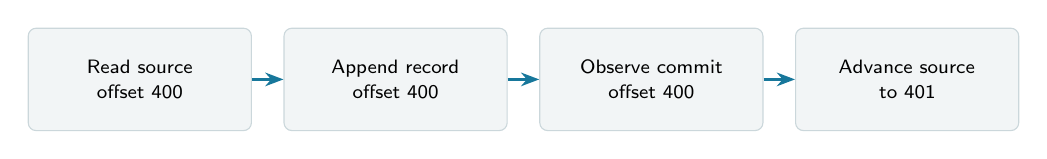
\begin{tikzpicture}[>=Stealth,every node/.style={font=\sffamily\fontsize{7.4}{9}\selectfont},b/.style={draw=thinrule,rounded corners=1mm,fill=papergray,text width=26mm,align=center,minimum height=13mm}]
\node[b](a){Read source\\offset 400};\node[b,right=4mm of a](b){Append record\\offset 400};\node[b,right=4mm of b](c){Observe commit\\offset 400};\node[b,right=4mm of c](d){Advance source\\to 401};
\draw[->,thick,steelblue](a)--(b);\draw[->,thick,steelblue](b)--(c);\draw[->,thick,steelblue](c)--(d);
\end{tikzpicture}\\{\fontsize{8}{9}\selectfont\color{inkgray}Figure 7.4. Durable acknowledgement must precede safe source advancement.}\end{center}
\begin{insight}\textbf{Correctness invariant}\par
For a single source partition, no source position greater than the last acknowledged committed position is permanently discarded from retry storage. The application may retry an uncertain submission; that must not silently multiply silver-layer records.\end{insight}
To test offsets, inject a failure at three boundaries: before submission, after submission but before acknowledgement, and after acknowledgement but before the upstream checkpoint. The first is a straightforward retry; the second and third test idempotence. Capture the exact destination and source states so a future maintainer can reproduce the outcome rather than rely on folklore.
\repo{P072: Java ingestion reference}{https://github.com/snowflakedb/snowflake-ingest-java}
\newpage
% PAGE 124 - 7.5.3
\topic{7.5.3}{Errors, disconnections, and reconnect design}
The client needs two failure classes. \emph{Retryable faults} include an interrupted network call, temporary throttling or unavailability. \emph{Non-retryable contract faults} include malformed or forbidden payloads, an invalid schema version or denied permissions until configuration changes. Infinite retries on a permanent error hide the cause and block useful work; immediate discard after a temporary timeout risks loss.

A sensible strategy applies bounded exponential backoff with jitter, a retry budget, explicit quarantine for poison records, and preserved source offsets. Enforce maximum queue memory: if the destination cannot keep up, pause or throttle the source rather than letting a process grow indefinitely. Log at least producer partition, source token, pipeline step, reason code, attempts, first-failure time and eventual outcome, without logging credentials or sensitive payloads.
\begin{lstlisting}[language=Python,caption={Illustrative retry decision, not a Snowflake SDK call.}]
if error.kind == 'TRANSIENT' and retries < limit:
    delay = min(max_wait, base_wait * 2 ** retries)
    schedule_retry(event_id, delay)
elif error.kind == 'CONTRACT':
    quarantine(event_id, error.reason)
else:
    stop_partition_and_alert(event_id)
\end{lstlisting}
\begin{whitebox}\textbf{Runbook: the channel reports an error}\par
(1) Freeze or slow upstream offsets. (2) Inspect channel error/status and event log without exposing payload secrets. (3) Find last committed offset. (4) Distinguish rejected rows from unacknowledged rows. (5) Reopen with the documented SDK recovery method. (6) Replay bounded source positions. (7) Compare raw and silver counts. (8) Record final incident timeline.\end{whitebox}
In the simulator, source offset~8 fails once and then succeeds. We record \emph{two attempts but one committed event}. That simple test is stronger than a screenshot showing a green connection. In a cloud exercise, preserve the client version, run identifier and actual channel-status output before asserting the system recovered.
\textbf{Check.} What happens if one poison event blocks a strictly ordered source partition? Propose a policy that preserves its identity and error while making later healthy events available, without lying about contiguous commit progress.
\newpage
% PAGE 125 - 7.6.1 and 7.6.2
\section*{7.6\quad Event ordering, duplicates, and late-arriving data}
\topic{7.6.1}{Arrival order is not event order}
Source systems produce \emph{event time}, transport imposes an arrival sequence, and the ingest client may commit asynchronously. These orderings are different. A sensor reading for 09:55 may arrive after 10:00 data because a device was offline, a retry waited, or a cloud region recovered. Sorting rows by ingest timestamp would make yesterday's correction appear newer than today's physical observation. Instead retain event time, original source partition/offset, ingest time, producer revision and an application-defined identity.
\begin{center}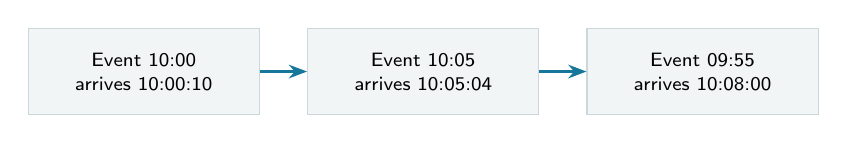
\begin{tikzpicture}[>=Stealth,every node/.style={font=\sffamily\fontsize{7.2}{8.8}\selectfont},b/.style={draw=thinrule,fill=papergray,align=center,text width=27mm,minimum height=11mm}]
\node[b](a){Event 10:00\\arrives 10:00:10};\node[b,right=6mm of a](b){Event 10:05\\arrives 10:05:04};\node[b,right=6mm of b](c){Event 09:55\\arrives 10:08:00};
\draw[->,steelblue,thick](a)--(b);\draw[->,steelblue,thick](b)--(c);
\end{tikzpicture}\\{\fontsize{8}{9.2}\selectfont\color{inkgray}Figure 7.5. Physical observations can arrive out of event-time order.}\end{center}
\topic{7.6.2}{Duplicates and idempotent analytical writes}
A repeated network acknowledgement, a retried event or two overlapping source extracts may cause an input to appear more than once. Define the deduplication key by \emph{business identity}: for our case \texttt{(provider, technology, event\_utc)} together with a revision ordering. Raw bronze may intentionally retain duplicate deliveries; silver must represent the latest approved revision once. A source event ID alone is insufficient when a legitimate correction uses a new message ID.
\begin{lstlisting}[language=SQL,caption={Select approved latest revisions at the analytical grain.}]
SELECT * EXCLUDE rn FROM (
  SELECT *, ROW_NUMBER() OVER (
    PARTITION BY provider, technology, event_utc
    ORDER BY revision DESC, received_utc DESC
  ) rn FROM energy_events_bronze
  WHERE energy_mwh >= 0
) WHERE rn = 1;
\end{lstlisting}
Tie-breaking policy matters. If two events carry the same business key and revision but different values, select neither arbitrarily: quarantine the conflict or escalate based on the publisher contract.
\repo{P073: Kafka streaming demonstration}{https://github.com/Snowflake-Labs/sfguide-kafka-interactive-tables-streaming}
\newpage
% PAGE 126 - 7.6.3
\topic{7.6.3}{Late corrections, watermarks, and honest freshness}
A \emph{watermark} is a declared bound on how far event-time processing is expected to lag. It is not simply the maximum observed timestamp. Consider a five-minute aggregation that waits up to two additional minutes for stragglers. If a reading for 10:00 arrives at 10:09, the system needs an explicit correction policy: revise a historical aggregate, publish an adjustment record, or reject it after a documented business cutoff. Every choice affects downstream trust.

For Finland energy reporting, retain UTC timestamps in the transport and fact grain; convert to \texttt{Europe/Helsinki} only for display or reporting periods with daylight-saving awareness. A local hour may be skipped or repeated around the daylight-saving transition. A source event with a local clock string but no offset is ambiguous on such dates and needs publisher rules, not a guessed conversion.
\begin{whitebox}\textbf{Three separate notions of late}\par
\emph{Transport late:} it was published promptly but queued. \emph{Publisher late:} the source only sent it after the measurement. \emph{Correction late:} the publisher issues a higher revision after downstream consumers had finalized a value. A single ingestion-lag number does not diagnose all three.\end{whitebox}
\begin{lstlisting}[language=Python,caption={Synthetic event age (seconds), not a service benchmark.}]
event_time = 0       # baseline UTC epoch in a toy clock
visible_time = 485   # illustrative late observation
age_seconds = visible_time - event_time
assert age_seconds > 300
\end{lstlisting}
Our lab retains one synthetic 09:55 observation arriving after 10:00 data. That late event increases the maximum event-to-bronze-visibility age even though it might have been ingested promptly after publication. For KPI reporting, measure the lag from the appropriate contractual clock and report late-data revisions separately.

\textbf{Production check.} Define a publishable hourly total when 99.9\% of expected interval keys arrive by minute~4, but a late correction is permitted for 48 hours. Record whether the displayed result is preliminary or finalized, and ensure analysts can identify version changes. \emph{Fast and correct} can mean versioned, not frozen.
\repo{P074: CDC plus Snowpipe pattern}{https://github.com/machkuma/aws-dms-s3-snowflake-cdc-snowpipe}
\newpage
% PAGE 127 - 7.7
\section*{7.7\quad Schema changes and failure recovery}
\topic{7.7.1}{Versioned payload mapping}
A new optional quality flag may be backwards compatible, while changing \texttt{energy\_mwh} into \texttt{energy\_kwh} is a semantic breaking change despite valid JSON. Accept only documented schema versions, preserve the untouched message and keep conversion rules in a tested mapper. Route unknown versions to a quarantine table until reviewed. Chapter~6's missing-versus-null checks remain essential in a continuous feed, where a bad schema can arrive thousands of times before somebody notices.
\topic{7.7.2}{Interrupted ingestion and state recovery}
A restart needs a known good source cursor and an independent destination commit record. Restore client identity, inspect named-channel status if supported, reconcile last committed positions, and replay the overlap needed to cover uncertain acknowledgement. Never advance the upstream cursor based solely on a client-side ``request sent'' message. For multi-partition sources, track independent progress; a single global counter can mask one stalled partition.
\topic{7.7.3}{Replay, quarantine, and safe cutover}
Backfills can interact with live traffic. Choose a bounded event range, preserve original event IDs and revision numbers, and make the silver merge idempotent. Quarantine records require an explicit disposition: reprocess after a mapper fix, replace from an authoritative snapshot, or mark irrecoverable with a signed reason. Do not silently drop them to make the dashboard healthy.
\begin{whitebox}\textbf{Failure injection matrix}\par
\textbf{Disconnect before send:} retry from source. \textbf{Commit uncertain:} verify channel progress, then replay safely. \textbf{Schema mismatch:} quarantine with version and field. \textbf{Duplicate delivery:} retain bronze provenance but prevent duplicate silver totals. \textbf{Late revision:} update the relevant analytical interval with an audit trail.\end{whitebox}
\textbf{Check.} A live feed begins publishing \texttt{unit='kWh'} without incrementing its schema version. Design the alarm, containment, replay and backfill steps that prevent an unnoticed thousandfold reporting error.
\repo{P075: Stream data generator}{https://github.com/Snowflake-Labs/simstreamer}
\repo{P076: Multi-service streaming reference}{https://github.com/Murataydinunimi/Real_Time_Streaming_Kafka_Airflow_DBT_Snowflake_ELK-Stack}
\newpage
% PAGE 128 - 7.8
\section*{7.8\quad Openflow and connector-based ingestion overview}
\topic{7.8.1}{When connectors are useful}
A purpose-built connector can own source polling, authentication, snapshot/CDC semantics, schema discovery and transformations that would otherwise take many lines of custom code. Its value is a maintained operational contract, not a magical guarantee that every row is correct. Evaluate connector lag, replay support, source permissions, observability, dependency lifecycle and change handling just as you would a bespoke consumer.
\topic{7.8.2}{Openflow deployment boundaries}
Snowflake Openflow provides managed integration workflows with deployment options including Snowpark Container Services-hosted runtimes and bring-your-own-cloud arrangements. A deployment contains runtimes, and a runtime executes one or more integration flows according to supported configuration. Do not assume the same integration features, preview status or runtime controls across deployment generations and cloud regions. The currently documented platform includes generation-specific limitations and some preview configuration features.
\topic{7.8.3}{Infrastructure, observability, and hidden costs}
Openflow can add running control-plane/compute-pool costs, per-runtime compute, ingestion credits, logging/telemetry and external transfer or CDC warehouse charges. An idle-looking flow may still incur compute-pool costs if its management resources remain running. Separate an \emph{integration demo} from the cheapest way to ingest a small periodic dataset. Before choosing Openflow, compare a minimal direct Snowpipe integration on identical acceptance criteria.
\begin{whitebox}\textbf{Connector review questions}\par
Does it support our database and precise CDC version? Can it recover after a multi-hour outage without snapshots duplicating rows? Who owns schema evolution? Which components keep billing when paused? What credentials are required? Can we export complete source offsets and raw events if the service is replaced?\end{whitebox}
\textbf{Example choice.} A PostgreSQL transactional source with ongoing CDC and multiple tables may justify an Openflow connector. A single weekly public energy CSV probably does not. Prefer the design with the least operational burden that meets measurable freshness, security and traceability requirements.
\repo{P021: Openflow on SPCS reference}{https://github.com/Snowflake-Labs/sfguide-getting-started-with-openflow-spcs}
\repo{P077: Openflow structured pipeline}{https://github.com/Snowflake-Labs/openflow-structured-data-pipeline-demo}
\repo{P078: Openflow PostgreSQL CDC}{https://github.com/Snowflake-Labs/sfguide-getting-started-openflow-postgresql-cdc}
\newpage
% PAGE 129 - 7.9.1 and 7.9.2
\section*{7.9\quad Latency, monitoring, throughput, and cost}
\topic{7.9.1}{Measure the full event-to-table path}
Measure pipeline stages separately: source observation, source publish, broker receipt, client read, Snowflake query visibility and silver readiness. Set clocks to UTC; record their precision and synchronization error. A message that is three minutes old at source publication cannot be fixed solely by changing the ingest product. Conversely, if publish-to-visible grows under pressure, inspect queue depth and client backlog before changing SQL transformations.
\begin{lstlisting}[language=SQL,caption={Freshness query against an approved raw table.}]
SELECT technology,
 DATEDIFF('second', event_utc, received_utc)
   AS source_age_seconds
FROM energy_telemetry_raw
WHERE event_utc IS NOT NULL;
\end{lstlisting}
\textbf{Measurement caveat:} \texttt{received\_utc} is a stored column, not proof of the query-visible timestamp. Use a separately recorded acknowledgment, controlled probe query, or documented channel metric to bound ingest visibility in a real benchmark. Instrument silver completion independently. For p95/p99, report sample count and the observation window, not only a representative screenshot.
\topic{7.9.2}{Throughput, backlog, and backpressure}
Define upstream offered rate \(\lambda\) and sustained downstream service rate \(\mu\). When \(\lambda>\mu\) for long enough, backlog grows regardless of optimistic average latency claims. Little's law relates long-run mean items-in-system \(L\), throughput \(\lambda\), and residence time \(W\) under stable conditions: \(L=\lambda W\). Use it diagnostically, not as an excuse to assume stationarity during an outage.

\begin{whitebox}\textbf{Alert example}\par
Alert if the oldest uncommitted source offset ages beyond the freshness objective for three consecutive evaluation windows, or if one partition stops advancing while others continue. Join this to acceptance/quarantine rates; a silent reduction in accepted rows can make throughput look ``fast'' while dropping data.\end{whitebox}
\textbf{Check.} A client handles 500 messages/s but the source produces 650 messages/s for 10 minutes. What backlog accumulated \emph{ignoring retries}? Why is an average ingest latency measured before the peak uninformative about recovery time?
\newpage
% PAGE 130 - 7.9.3 and sources
\topic{7.9.3}{Separating ingestion billing from pipeline economics}
Compare costs using the account's actual service consumption table and a time-bounded meter export. File-based Snowpipe usage can be examined in \texttt{PIPE\_USAGE\_HISTORY} in the Snowflake Account Usage schema, which has reporting latency. High-performance Snowpipe Streaming is metered separately according to its documented throughput-oriented model. Traditional warehouses, connector runtimes and downstream transformations are separate billable resources. Resource monitors that stop user-managed warehouses do not, by themselves, cap every serverless ingestion or connector charge.
\begin{lstlisting}[language=SQL,caption={Auditable file-based Snowpipe meter query; requires privileges.}]
SELECT TO_DATE(start_time) AS usage_day,
       pipe_name,
       SUM(credits_used) AS credits_used,
       SUM(bytes_billed) AS bytes_billed
FROM snowflake.account_usage.pipe_usage_history
WHERE start_time >= DATEADD(day,-7,CURRENT_TIMESTAMP())
GROUP BY 1,2 ORDER BY 1,2;
\end{lstlisting}
This query reports service usage, not end-to-end energy-dashboard cost. Add storage, query warehouses, stream processing, orchestration, network and on-call cost before comparing architectures. Document reporting lags; do not describe incomplete last-hour metering as zero charges.
\begin{whitebox}\textbf{Five metrics to keep}\par
(1) Accepted input events/s; (2) p95 event-to-bronze age; (3) p95 event-to-silver readiness; (4) partition offset lag and oldest retry age; (5) ingestion \emph{and} downstream credits per million approved observations. Always report quarantines separately.\end{whitebox}
\textbf{Reading trail and status.} Snowflake documentation checkpoint: 22 October 2026. Full links appear in the companion README and the references here; functionality, prices and edition limitations may change. Primary references: \href{https://docs.snowflake.com/en/user-guide/data-load-snowpipe-auto}{Snowpipe auto-ingest}; \href{https://docs.snowflake.com/en/sql-reference/sql/create-pipe}{CREATE PIPE}; \href{https://docs.snowflake.com/en/user-guide/snowpipe-streaming/snowpipe-streaming-high-performance-comparison}{streaming architectures}; \href{https://docs.snowflake.com/en/user-guide/snowpipe-streaming/snowpipe-streaming-operations}{named-channel recovery}; \href{https://docs.snowflake.com/en/user-guide/data-integration/openflow/cost-spcs}{Openflow costs}; and \href{https://docs.snowflake.com/en/user-guide/data-load-snowpipe-billing}{file Snowpipe costs}. No live cloud ingest or cost benchmark was performed.
\repo{P079: Event streaming presentation reference}{https://github.com/Snowflake-Labs/Summit2025-DE214}
\repo{P080: Community end-to-end streaming demo}{https://github.com/JeetThakore/Real-Time-Heart-Rate-ELT-Pipeline-Kafka-Streaming-to-Snowflake-with-Airbyte-dbt-Dagster-Tableau}
\newpage
% PAGE 131 - 7.L.1 and 7.L.2
\section*{7.L\quad Guided lab: a failing energy telemetry feed}
\topic{7.L.1}{Inputs, environment, permissions, and cost}
The companion's \texttt{streaming\_simulator.py} runs with Python~3.10+ and the standard library only. It models one ordered source partition over nine synthetic events. An exact duplicate, a higher-revision correction, a late arrival, a negative measurement and a retry after transient failure are deliberately included. No network access, Snowflake account, API key or credits are required for the offline experiment.

The optional SQL files are \emph{integration templates}, not executed database scripts. Only run cloud components after an administrator approves a disposable schema, a narrowly scoped role, storage integration, region and cost limit. A file-based Snowpipe definition needs an actual authorized external stage; a high-performance streaming pipe needs a matching current SDK/REST client. Never publish secrets or assume a commented pipe template provides an event queue.
\topic{7.L.2}{Execute and inspect the deterministic experiment}
\begin{lstlisting}[language=bash,caption={From the extracted Chapter 7 lab folder.}]
python streaming_simulator.py --out output
python -m unittest -v test_streaming_simulator.py
\end{lstlisting}
Inspect \texttt{output/bronze.csv} and \texttt{output/silver.csv}. Bronze preserves eight accepted deliveries, including the duplicate and the older wind revision. Silver selects one approved revision for each (provider, technology, UTC interval) key. The negative reading goes to \texttt{output/quarantine.json}; the failure at source offset~8 is recorded in \texttt{attempts.json} before replay succeeds. The final source offset is committed only after a successful attempt.
\begin{center}\renewcommand{\arraystretch}{1.13}\begin{tabularx}{\linewidth}{@{}Xr@{}}\toprule
\textbf{Deterministic simulator output (offline)}&\textbf{Result}\\\midrule
Source records / delivery attempts&9 / 10\\
Accepted bronze / quarantined&8 / 1\\
Unique latest-revision silver facts&6\\
Silver total, MWh&66.000\\
Median / maximum event-to-visible age, seconds&27 / 485\\
Last safely committed synthetic offset&8\\\bottomrule
\end{tabularx}\\{\fontsize{8}{9.5}\selectfont\color{inkgray}Table 7.3. Measured from synthetic fixture clocks, not Snowflake.}\end{center}
\textbf{Failure interpretation.} The large maximum reflects a deliberately late observation, not necessarily a slow ingest service. Reporting it as Snowflake's p99 latency would be a serious measurement error. Distinguish accepted source delivery from published business readiness and document the assumed clock domains.
\newpage
% PAGE 132 - 7.L.3 and 7.L.4
\topic{7.L.3}{Assertions, diagnosis, replay, and cleanup}
The eight offline tests check row accounting; higher-revision precedence; total MWh; quarantine; retry/commit order; late-event detection; deterministic replay; and the no-failure baseline. The strongest invariants are: accepted bronze plus quarantined equals unique source messages; silver contains at most one approved latest revision per business key; replay does not increase the business total; and the committed source offset never skips an unprocessed failure.

If the count differs, inspect \texttt{attempts.json}. If energy total increases on a second run, inspect business-key deduplication and revision precedence. If freshness is negative, validate event and visibility clocks before treating the message as fast. \textbf{Cleanup:} remove the local \texttt{output/} directory; the lab creates no cloud resources. Cloud teardown must be approved separately after actual integration testing.
\topic{7.L.4}{Practice, architecture decision, and assessment}
\textbf{Foundation exercise.} Add a second duplicate delivery and assert that bronze count increases while silver count and total remain stable. \textbf{Practitioner exercise.} Add a late higher-revision correction for hydro and prove that the final energy total changes exactly once. \textbf{Production decision.} Design a rollout from hourly file loads to row-based streaming for an energy alarm. Specify source partitions, channel mode, credentials, safety limit, backpressure, clock measurements, reconciliation and rollback. Decide whether the extra speed is worth its operational obligations.
\begin{whitebox}\textbf{Assessment rubric (10 points)}\par
Architecture selection with measurable freshness (2); explicit source/target acknowledgment invariant (2); duplicate and revision-correction handling (2); quarantine and replay evidence (2); cost, privacy and cleanup plan (2). An architectural choice without source-offset safety cannot receive full marks.\end{whitebox}
\textbf{Key takeaways.} ``Continuous'' describes delivery, not guaranteed freshness; exactly-once semantics have a specified boundary; event-time ordering is distinct from arrival order; poison records need a named disposition; and costs include service-side compute, cloud plumbing and operating responsibility. Chapter~8 will consume this trusted bronze feed through Snowflake Streams, Tasks and Dynamic Tables, keeping ingestion and subsequent change processing as separate concerns.
\begin{insight}\textbf{Publishing verification gate.}\par
At print approval, confirm all cited APIs, region/edition constraints, ingest and channel costs, repository licenses and client versions; run selected SQL in a bounded Snowflake test account; capture execution IDs, date, actual usage and cleanup proof. The present chapter does \emph{not} claim those cloud tests were completed.\end{insight}

\end{document}
